\documentclass[a4paper, 12pt]{article}
\usepackage{titling}
\usepackage{array}
\usepackage{booktabs}
\usepackage{enumitem}
\usepackage{graphicx}
\usepackage{hyperref}
\usepackage{amssymb}
\setlength{\heavyrulewidth}{1.5pt}
\setlength{\abovetopsep}{4pt}
\setlength{\parindent}{0pt}
\graphicspath{{.}}

\usepackage[margin=1in]{geometry}

% Must be after geometry
\usepackage{fancyhdr}
\pagestyle{fancy}
\fancyhf{}
\rhead{NN Homework 2}
\lhead{P.Lukin, I. Vishniakou, E. Ovchinnikova}
\cfoot{\thepage}

\setlength{\droptitle}{-5em}

\title{Neural Networks  \\
				- Homework 2 -}
\author{Petr Lukin, Ivan Vishniakou, Evgeniya Ovchinnikova}
\date{Lecture date: 10 October 2016}

\begin{document}

\maketitle

\section{Mind map}

\begin{figure}[h]
  \centering
  \caption{S. Haykin, Neural Networks, chapter 2 (before 2.13). Mind map (a zoomed version of the map is attached as mindmap.png file).\label{fig:mindMap}}
  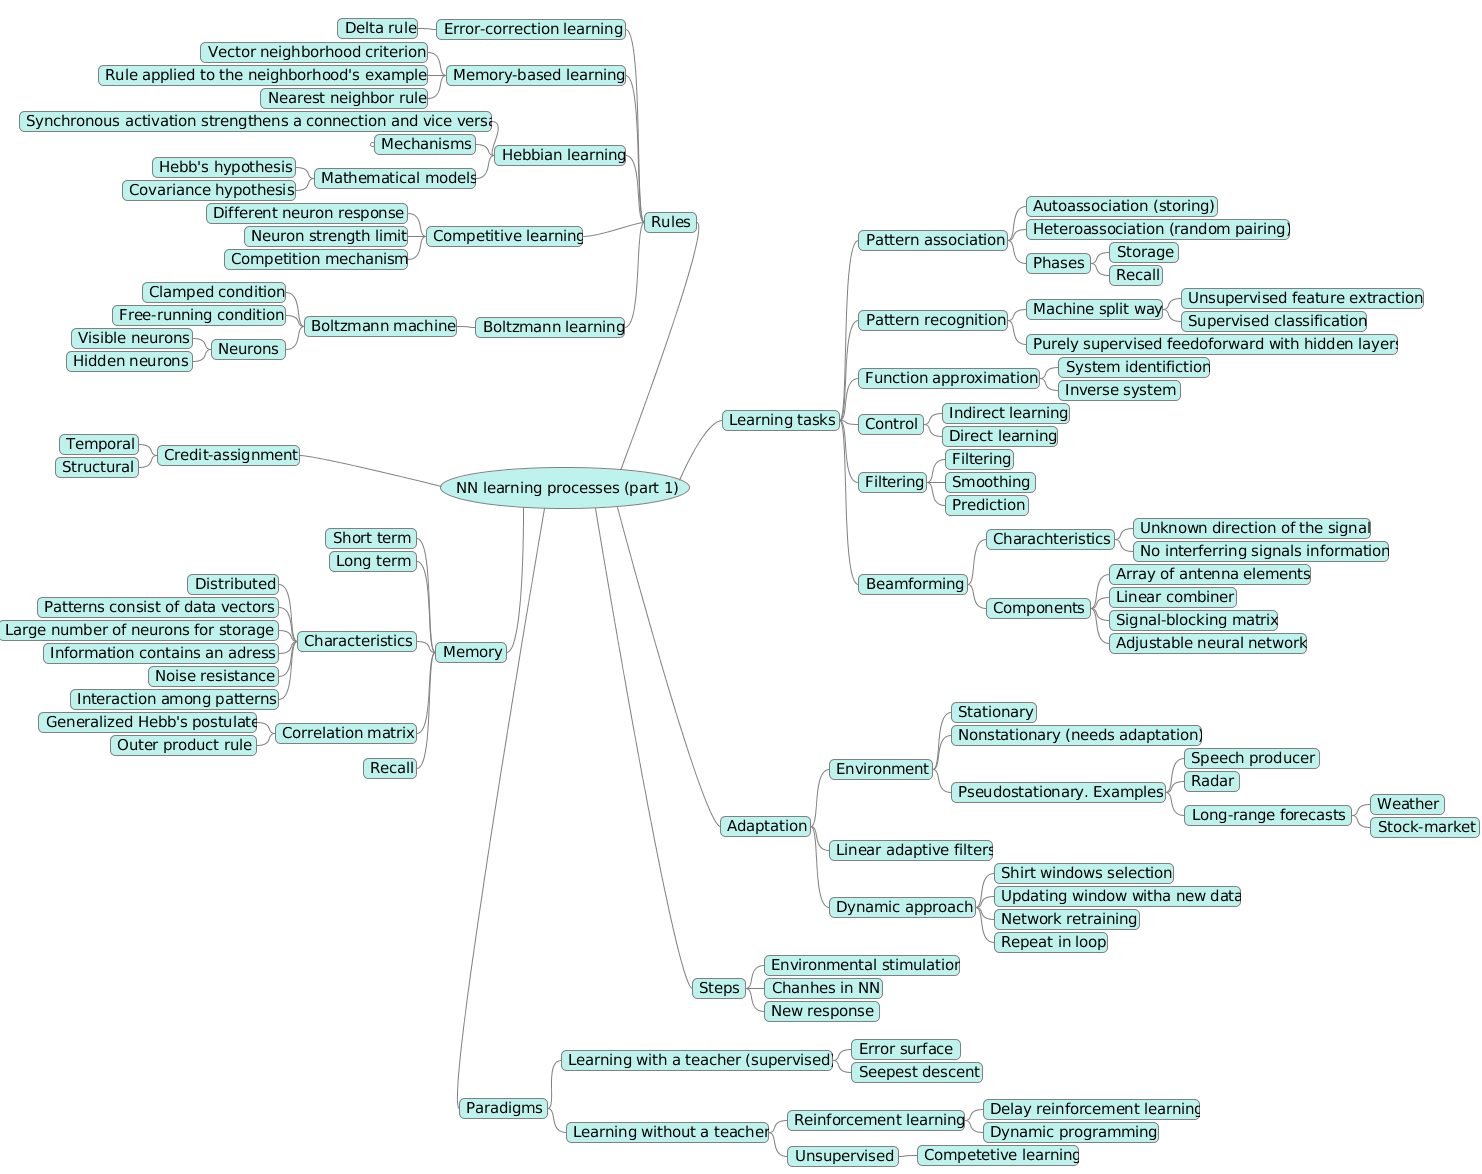
\includegraphics[width=1.0\textwidth]{mindmap}
\end{figure}

\section{Exercises}

\subsection{Exercise 1.13}

\subsection{Exercise 4}

Derive the Delta rule for two ADALINE neural networks depicted in Fig. \ref{fig:nn1}, Fig. \ref{fig:nn2}.

Solution:\\

1 neural network.\\

\begin{figure}[h]
  \centering
  \caption{Neural network 1. \label{fig:nn1}}
  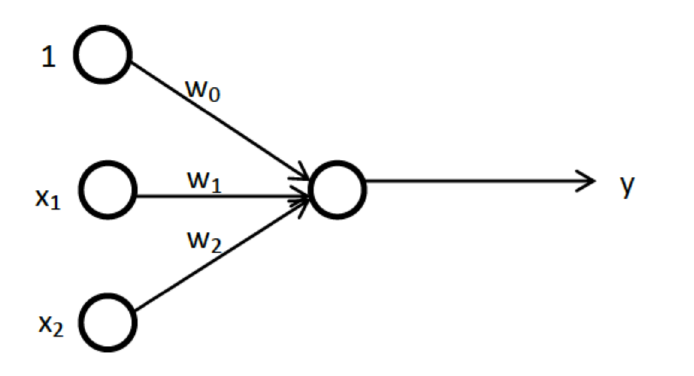
\includegraphics[width=0.5\textwidth]{nn1}
\end{figure}

Input: 	$\vec{x} = (x_0, x_1, x_2)$,  where $x_0 = 1$\\
Weights: 	$\vec{w} = (w_0, w_1, w_2)$\\
Output: $y = \vec{x} \vec{w} = w_0 + x_1w_1 + x_2w_2$\\

$e = d - y = d - (w_0 + x_1w_1 + x_2w_2)$, where d is a desired value.\\

$E(w) = \frac{1}{2}e^2$\\

Each $i^{th}$ weight with an should be moved in the direction $\frac{\partial E}{\partial w_i}$:\\

$\frac{\partial E}{\partial w_i} = x_i(d - (w_0 + x_1w_1 + x_2w_2))$\\

So, each step will change each weight by the following value:\\
$\Delta w_i = \eta x_i(d - (w_0 + x_1w_1 + x_2w_2))$,\\
where $\eta$ is a learning rate that should be chosen according to the specific of the certain case. It can be either a constant (0.5, 1, etc.) or variable, or adaptive.\\

Therefore the delta rule will take the following form:\\

$w_i^{new} = w_i^{old} + \eta x_i(d - (w_0 + x_1w_1 + x_2w_2))$\\

Neural network 2.

\begin{figure}[h]
  \centering
  \caption{Neural network 2. \label{fig:nn2}}
  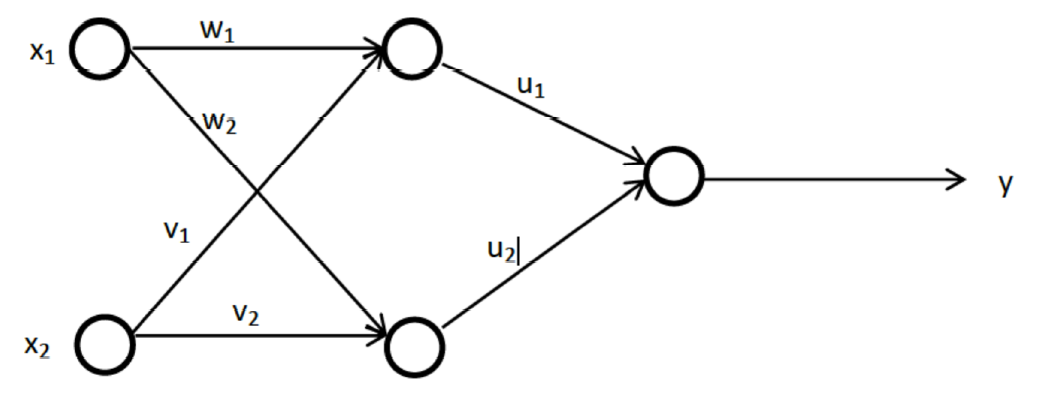
\includegraphics[width=0.6\textwidth]{nn2}
\end{figure}

Input: 	$\vec{x} = (x_1, x_2)$\\
Weights: 	$\vec{w} = (w_1, w_2)$, $\vec{v} = (v_1, v_2)$, $\vec{u} = (u_1, u_2)$\\
Activation function is linear, so:\\
Output: $y = u_1(x_1w_1 + x_2v_1) + u_2(x_1w_2 + x_2v_2)$\\

$e = d - y = d - (u_1(x_1w_1 + x_2v_1) + u_2(x_1w_2 + x_2v_2))$.\\

Each $i^{th}$ weight with an should be moved in the direction $\frac{\partial E}{\partial weight_i}$:\\

$\frac{\partial E}{\partial v_i} = x_1u_i(d - (u_1(x_1w_1 + x_2v_1) + u_2(x_1w_2 + x_2v_2))$\\

$\frac{\partial E}{\partial w_i} = x_2u_i(d - (u_1(x_1w_1 + x_2v_1) + u_2(x_1w_2 + x_2v_2))$\\

$\frac{\partial E}{\partial u_i} = (x_1w_i + x_2v_i)(d - (u_1(x_1w_1 + x_2v_1) + u_2(x_1w_2 + x_2v_2))$\\

So, each step will change each weight by the following value:\\

$\Delta w_i = \eta_w x_1u_i(d - (u_1(x_1w_1 + x_2v_1) + u_2(x_1w_2 + x_2v_2))$,\\
$\Delta v_i = \eta_v x_2u_i(d - (u_1(x_1w_1 + x_2v_1) + u_2(x_1w_2 + x_2v_2))$\\
$\Delta u_i = \eta_u (x_1w_i + x_2v_i)(d - (u_1(x_1w_1 + x_2v_1) + u_2(x_1w_2 + x_2v_2))$\\

Therefore the delta rule will take the following form:\\

$w_i^{new} = w_i^{old} + \eta x_i(d - (w_0 + x_1w_1 + x_2w_2))$\\
$v_i^{new} = v_i^{old} + \eta_v x_2u_i(d - (u_1(x_1w_1 + x_2v_1) + u_2(x_1w_2 + x_2v_2))$\\
$u_i^{new} = u_i^{old} + \eta_u (x_1w_i + x_2v_i)(d - (u_1(x_1w_1 + x_2v_1) + u_2(x_1w_2 + x_2v_2))$\\


\end{document}
